\section{Methods}

\subsection{Sampling Images}

The collection of lifelog images distributed for the NTCIR-12 conference far exceeds the possibility of annotating every image. The collection is very large, containing around 90,000 images. It is certainly unfeasible to annotate every image four times (for each annotation methodology), so sampling is a necessity. Previous work~\citep{scells2016qut} identified a way of clustering lifelog images based on temporal information and image histograms. After clustering images, a rough sampling technique can be performed which involves selecting one image at random from each cluster. Given more time, it would be worthwhile investigating other image similarity measures (such as those used by the LEMoRe team at NTCIR-12~\citep{de40lemore}) to possibly produce a more uniformly distributed sample set.

This sampling process reduces the total number of images needed to annotate to around 16,000. This is slightly more feasible and, intuitively, should be enough to perform some analysis on. The sampled images are uploaded into a database, ready to be annotated. This subset represents the number of annotations which will be distributed as a test collection, and the images in that test collection which have been annotated. For future work, a combination of clustering and matching images to relevant topics might be a better option, as there will most likely be many irrelevant annotations. There may also be no annotations which are relevant to a topic as well, since the sampling is somewhat random. This makes the process less than idea, but will serve as a proof of concept for further research.

\subsection{Collecting Annotations}

A test collection of accurate lifelog annotations to go along with the images is crucial for developing an effective information retrieval system or classification system. The outcomes of this thesis will be the collection of all annotations, as well as the annotation methodology or combination of methodologies which are found to be the most effective for search. This is important since annotations are only evaluated on their effectiveness for searching lifelog images, as opposed to the best annotation methodology for classifying images. This is why all of the collected annotations are made available, since the use cases for them are not limited to just typical search.

\subsubsection{Architecture}
A set of web application interfaces are used for the collection of annotations. Each interface will provide a means for an annotator to assign the respective annotation type to an image from the list of unannotated images. The architecture of these interfaces consists of:
\begin{enumerate}
    \item A database to store the annotations and the collection of images. The database will also store information about each user performing the annotations and who annotated which image. This ensures there is a record of who annotated each image, and allows for some type of analysis to be performed at a later stage.
    \item A web server that handles the "business logic". This web server exposes some password protected RESTful services that applications can hook into.
    \item Some web pages which consume the API provided by the web server and present view logic. This is the layer that annotators will interact with directly. Each interface will be one of these views.
\end{enumerate}

Annotations are inserted into the database, which can then be exported and used further down the line for other purposes such as  classifier training and evaluation. 

\subsubsection{Annotation Methodologies}

There are four annotation types under investigation. Each one is very different to the last and some interesting comparisons will hopefully be able to be drawn. There have been no studies into the most effective methodology or set of methodologies for annotating lifelog images. It would be nice to investigate more than four, however due to time constraints this is inconceivable. The annotation methodologies in question are: \textbf{textual}, \textbf{tags}, \textbf{relevance assessment} and \textbf{reverse query}. 

Each type of annotation is collected in a very similar way. An expert annotator is shown an image from the sampled collection and is asked to provide an annotation (or in the case of relevance assessment, multiple annotations) for the image. The interfaces used for collecting annotations are pictured and described as follows:

\newpage
\textbf{Textual}

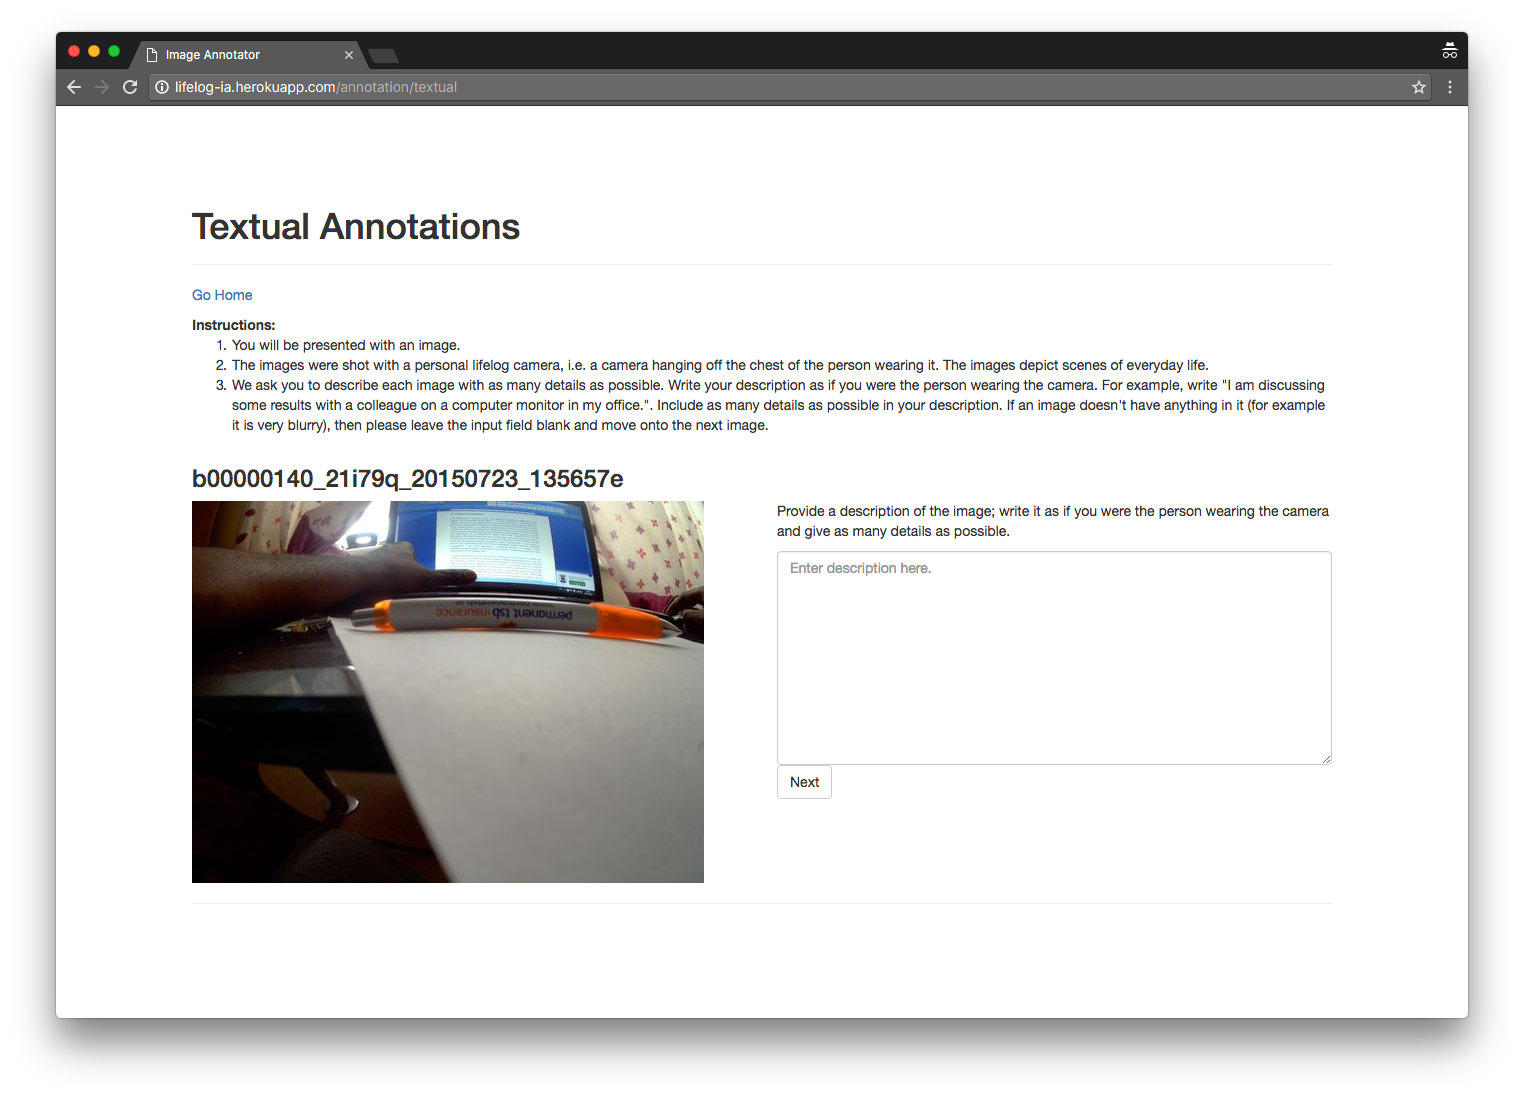
\includegraphics[width=\textwidth]{images/text-interface}

Here, annotations are collected using a text box. Free form text can be entered by the expert annotator. Textual queries should contain semantic information about an image, and should describe the image with as much detail as possible. These annotations are very similar to a textual document in a typical web search engine, which is why they were selected as one of the methodologies to investigate. These annotations may not be the best for training an image classifier, but it is hypothesised that they will perform the best in a search task.

Textual annotation are the most time consuming annotation type to collect. Many images contain two or more highly relevant events or `important' objects. Describing these can take annotators up to several minutes each. This is opposed to all the other annotation methodologies where most images can be annotated in a minute or less.

\newpage
\textbf{Tags}

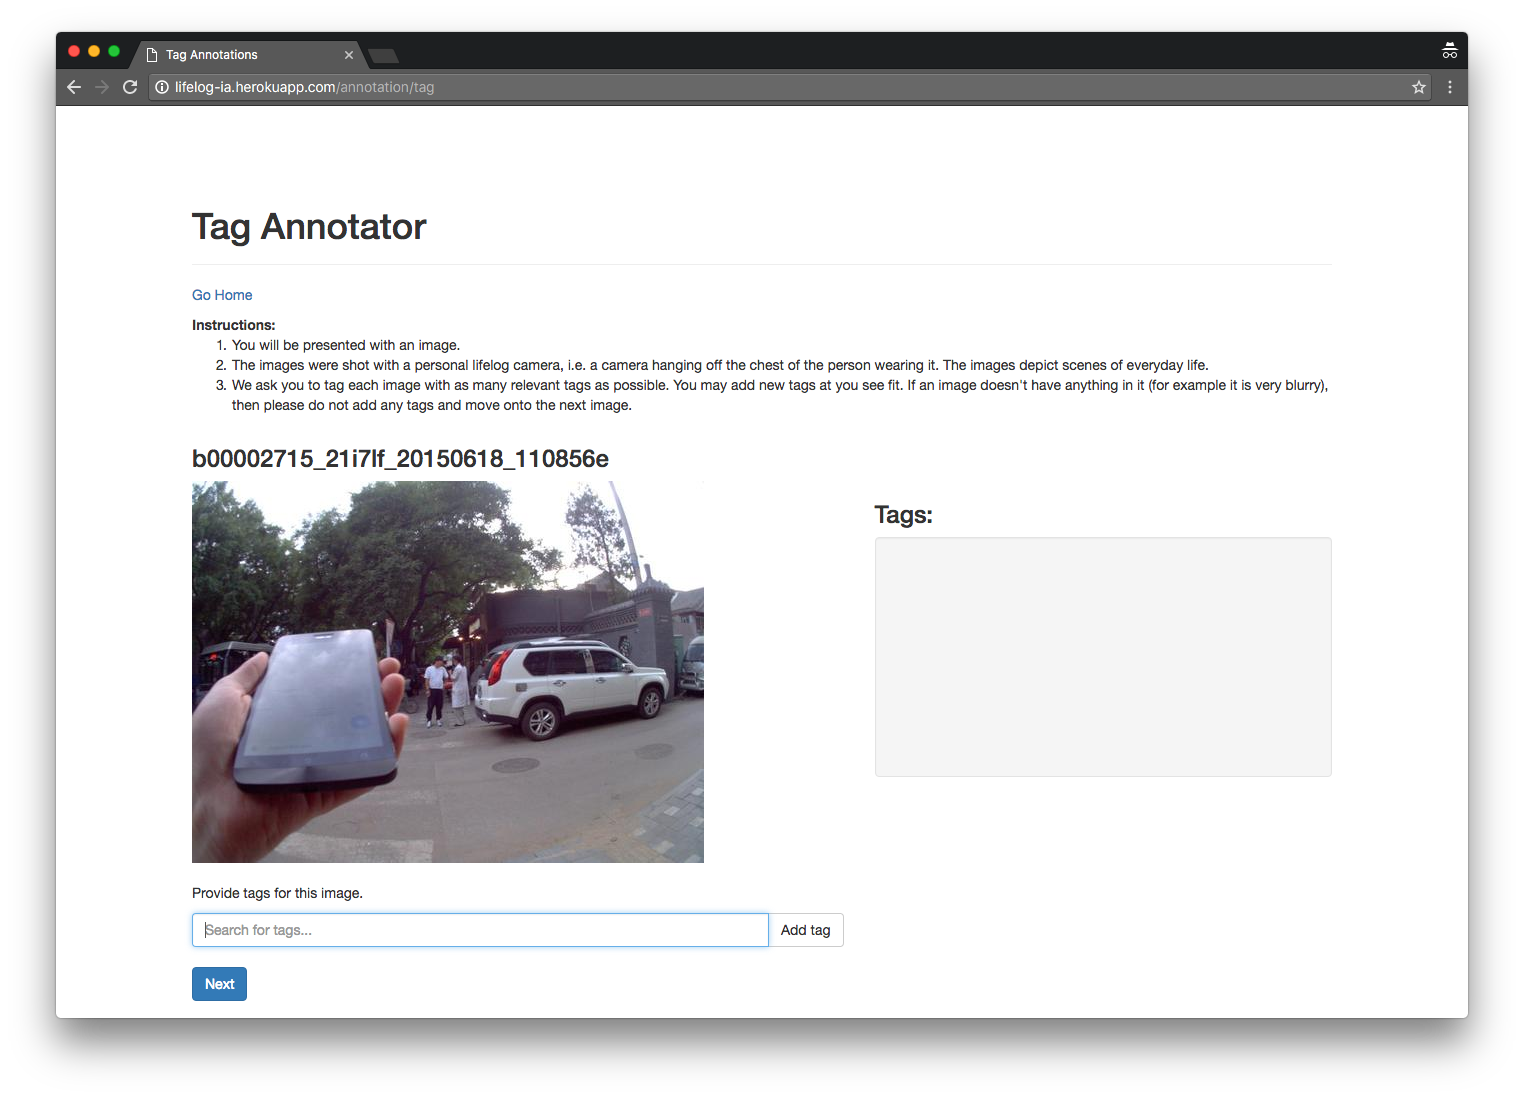
\includegraphics[width=\textwidth]{images/tag-interface}

Tags are collected through a specifically designed interface. These vocabulary of tags is created from previously added tags, meaning the list of tags available is arbitrary and can be expanded. In terms of evaluation, tags may be the opposite of textual annotations; intuitively tags should be the best at training an image classifier and are expected to perform the worst when embedded a search task. Tags, however, may be very good at boosting the performance of other annotation types in the search task when combined. For instance, searching on the text \textit{and} tags fields may increase the scores of text annotation alone.

It is predicted that the collection of tags will be very fast. Given that similar tags are also presented to the annotator, so they do not need to type the full description out each time, this will cut the time down significantly. Collecting tags will be useful for later on in the project when the concepts for relevance assessment will be determined. These concepts will be created based off a distribution of the number of times a tag is used, and will also incorporate some notion of relevance to the NTCIR-12 topics (since the collection of images relates to the topics).

\newpage
\textbf{Reverse Query}

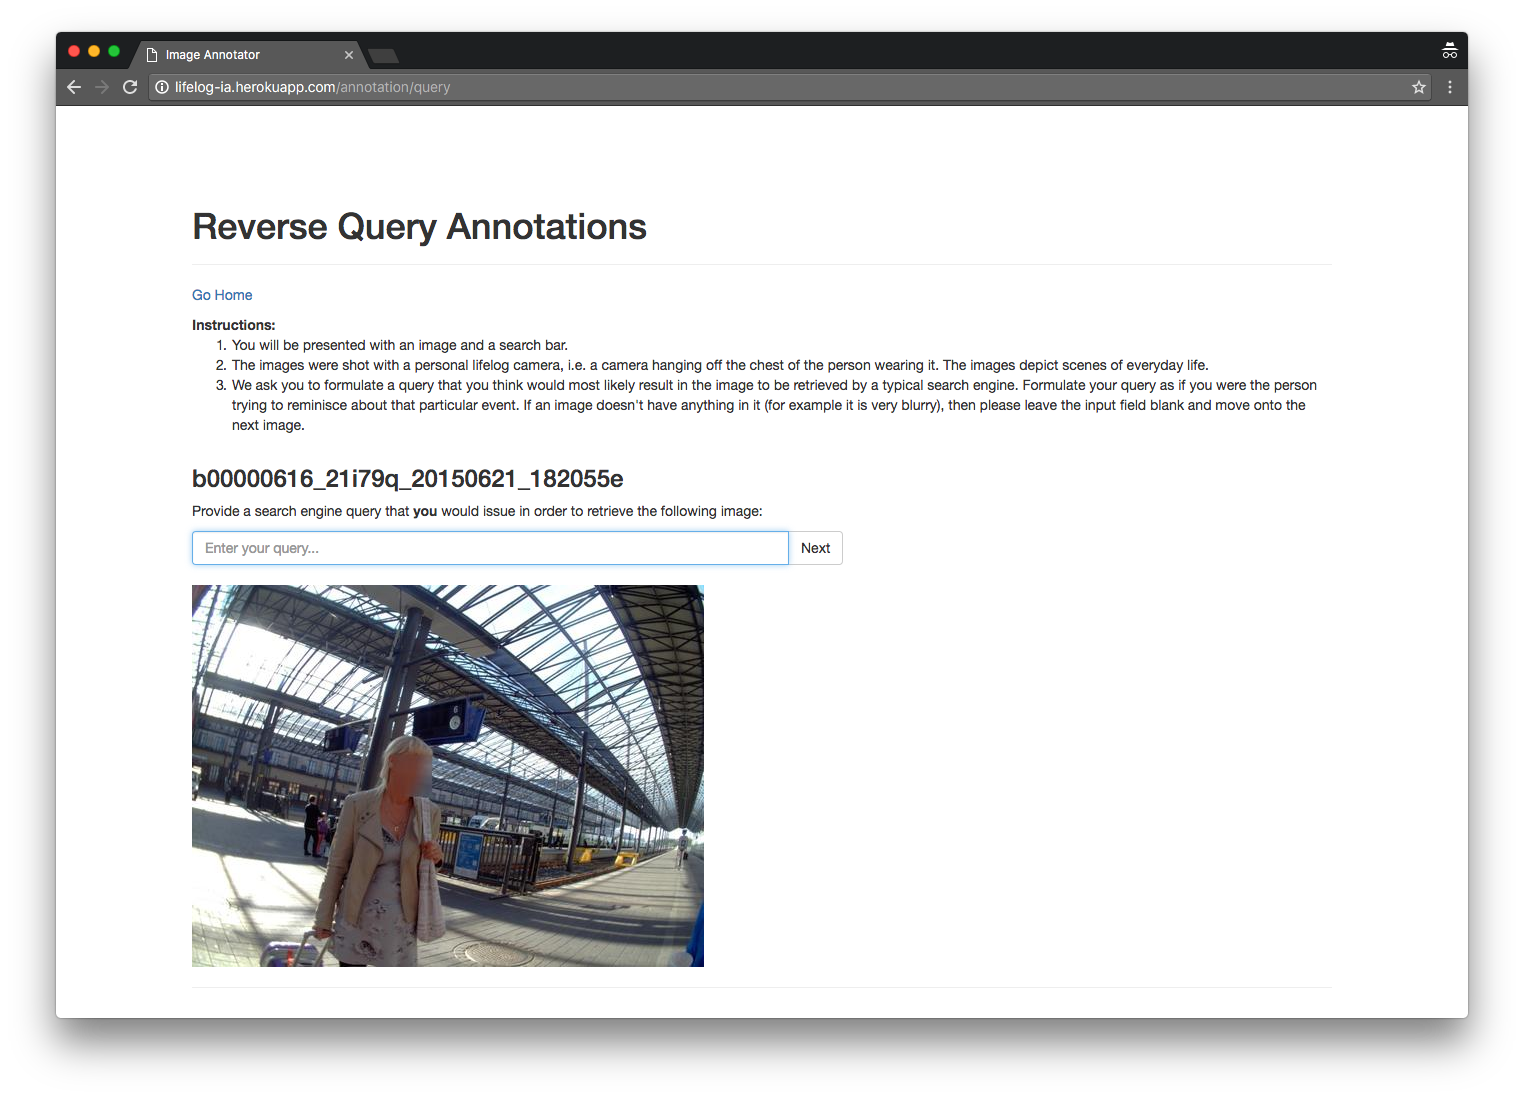
\includegraphics[width=\textwidth]{images/query-interface}

In this interface, user queries are collected by presenting an image taken from the lifelog camera and asking the annotator to provide a query with what they expect to be returned by a typical search engine. This is a relatively new and novel way to annotating \textit{any} type of document or image \todo{citation needed} and therefore it is unknown how well the collected queries will perform in search or for training an image classifier. The level of detail in these annotations will be very low, since most queries are very short \todo{citation needed}; therefore when training an image classifier, it is expected that queries will not do very well.

Much like tags, this annotation type will be very easy to collect. Formulating a query for an image should not take a significant amount of time. There is the problem of bias \todo{Is there really? I should investigate this further}

\newpage
\textbf{Relevance Assessment}

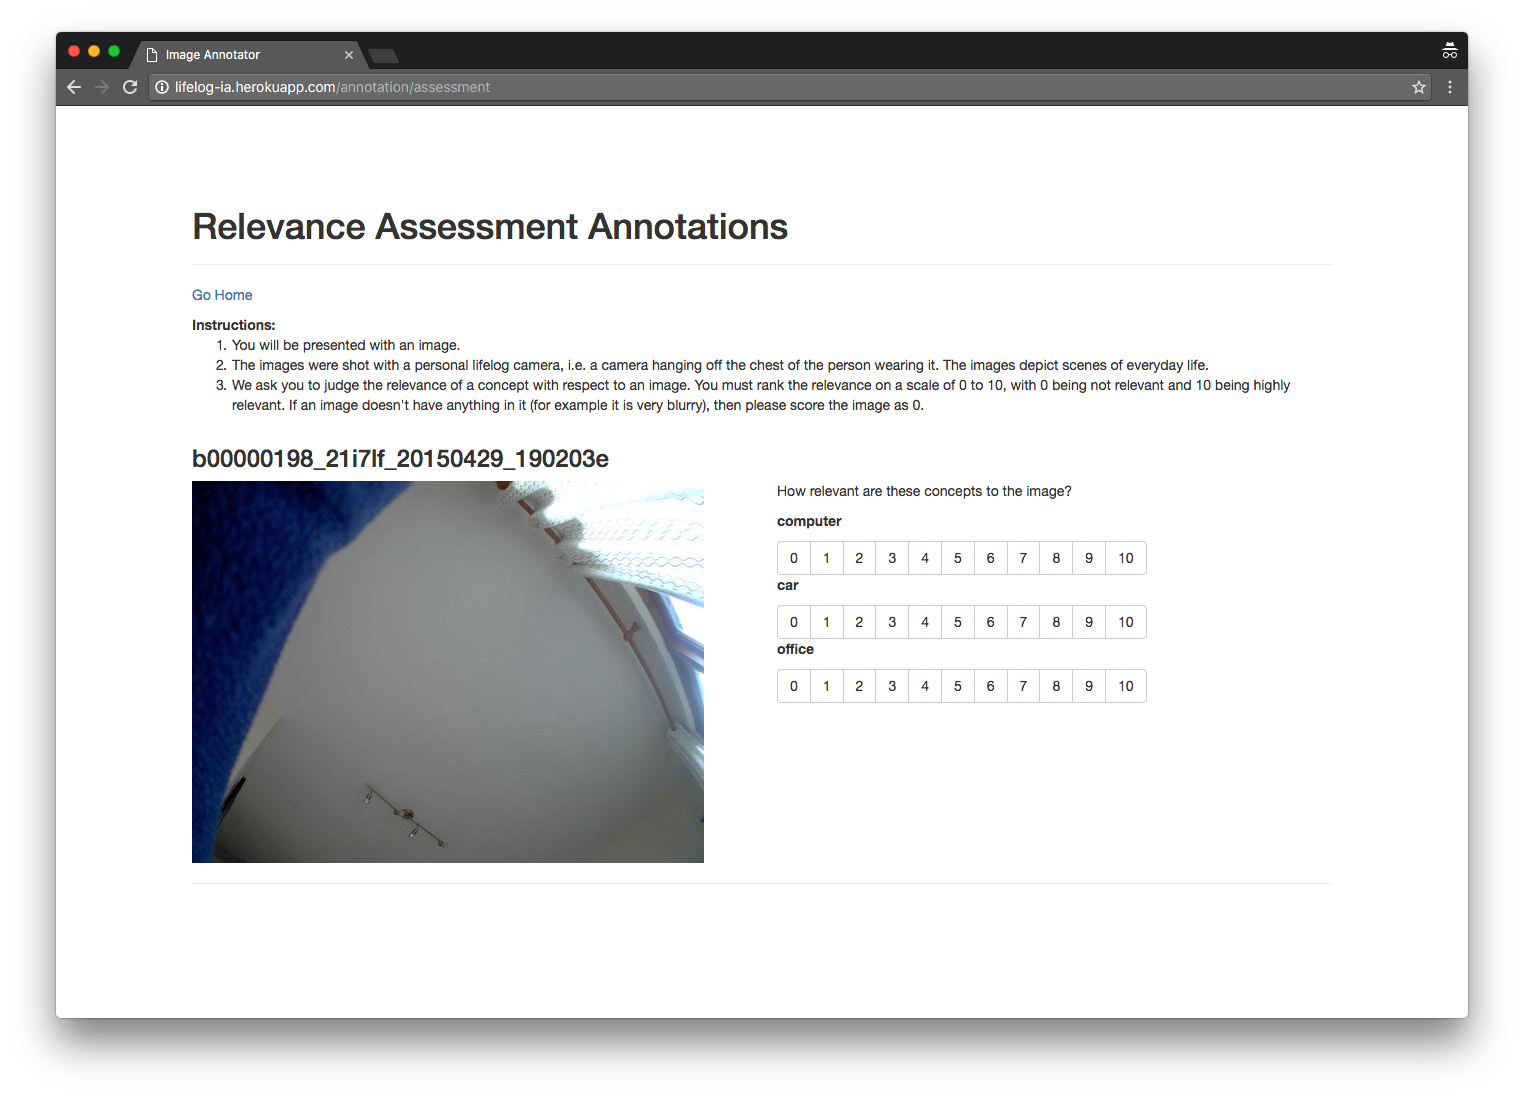
\includegraphics[width=\textwidth]{images/rel-ass-interface}

Relevance assessment involves presenting an annotator with an image, and asking them to judge how relevant a concept is to the image. These annotations will be collected last, since the list of concepts does not exist yet. It was originally planned that the concepts would be formed using a process that involved the topics from the NTCIR-12 data set. This, however, is not ideal, since the clustering process mentioned above may filter out all of the images which are relevant to a topic. It is for this reason that this annotation type will be collected last. The concepts will be formed from a combination of the previous annotations.\todo{expand on why}

\todo{I need to talk about collecting the annotations}

\subsection{Evaluation}

\subsubsection{Evaluating Annotations}

Annotations are evaluated through statistical analysis. This will determine which annotation or combination of annotations are most effective for searching lifelog images. There is little research in evaluating test collections, however the work here will build upon previous work done by \todo{citation needed}.

A set of runs will be produced in an ad-hoc, TREC style evaluation. Every combination of annotation will be an independent run. We would like to test the combinations of annotations because, for example, the combination of tags and queries might produce better results than simply the tags or query annotations alone.

Evaluation is performed through a custom-built framework. A Java RESTful application wraps an Elasticsearch instance and performs evaluation through this. Runs are produced by issuing bulk queries to the application. The result is a set of query relevance sets (qrels) that can be evaluated through the use of trec\_eval.

\begin{enumerate}
    \item Elasticsearch is used as the information retrieval system
    \item A RESTful Java application exposes an API to add and retrieve annotations to an Elasticsearch index, as well as to perform TREC runs
    \item trec\_eval is used to evaluate the runs produced by the previous system
    \item Items two and three are repeated for every combination of annotation types using a script
\end{enumerate}

This will identify which annotations out of the four tested are the most effective for searching lifelog images. What is arguably more important is evaluating how good the best annotations are as a test collection for lifelog images. A test collection which does not suit the needs of the topics being tested is not very helpful. In doing this, it will determine if the annotations are a good fit for testing a search engine system as a whole.

\subsubsection{Evaluating The Test Collection}

It may not just be good enough to evaluate how good the annotations are, it is also worthwhile to evaluate the test collection of annotations as a whole. The subset of `gold standard' annotations are the manual human-annotated images. The rest of the annotations in this collection will be automatically generated using a state-of-the art machine learning image classification approach~\citep{karpathy2015deep}.
